% ЕМТ 2024, V клас — точен LaTeX препис от официалните файлове в Klasirane.com.
% Условия: https://klasirane.com/api/competitions/EMT/All/2024/5%20%D0%BA%D0%BB/probs
% SHA-256 (условия): 10acfdda5bb290931132c12f2f6613f9ccd1d99f04f8f587512014a35d92522a
% Решения: https://klasirane.com/api/competitions/EMT/All/2024/5%20%D0%BA%D0%BB/sol
% SHA-256 (решения): 8dc6786710777ec610a468ebbc972c55bf4c4ab64ed6b2d138ebc97c9b0cb087
% Точковите оценки, правописът, формулировките и видимите печатни грешки са запазени от източника.
% Файлът с условията е сканирано изображение; видимите страници са проверени пряко.
% Фигурите са извлечени без промяна от отделните JPEG обекти в официалния PDF с решенията.

Задача 5.1. През квадратна градина $ABCD$ прекарали алея, както е показано на чертежа. Алеята разделила $ABCD$ на две правоъгълни градини. Страните на градините, измерени в метри, са естествени числа. Площта на северната градина е с 507 кв.м по-голяма от площта на южната. Третината от северната градина и половината от южната градина засадили с пипер, а останалата част от градините – с домати. Оказало се, че с пипер са засадили общо 559 кв.м.

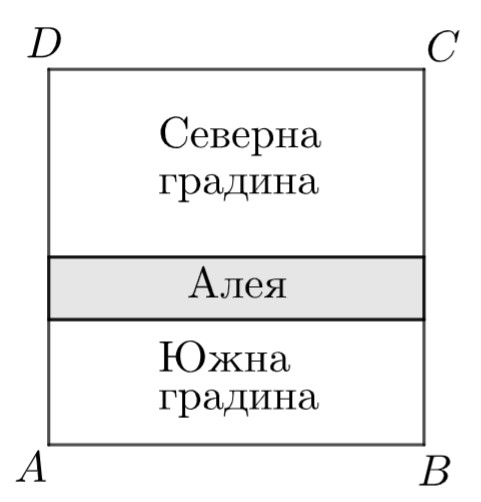
\includegraphics[max width=0.48\textwidth, alt={Квадратната градина ABCD, разделена на северна градина, алея и южна градина}, center]{assets/5-1-garden.jpg}

а) Колко квадратни метра общо са засадили с домати?

б) Колко квадратни метра е площта на алеята?

Решение. Нека третината от северната градина има площ $x$ кв.м, а половината от южната градина има площ $y$ кв.м. С пипер са засадили общо
$$x+y=559\text{ кв.м.}$$
Площта на северната градина е $3x$ кв.м, а на южната градина е $2y$ кв.м. Тогава
$$3x-2y=507.$$
Като удвоим първото равенство и съберем с второто, получваме, че $5x=1625$, т.е. $x=325$. Следователно $y=559-325=234$.

Площта на северната градина е $3\cdot325=975$, а площта на южната градина е $2\cdot234=468$; общо $975+468=1443$ кв.м.

а) С домати са засадили $1443-559=884$ кв.м.

б) Страната на квадрата е общ делител на площта на северната градина и площта на южната градина. Тъй като $\operatorname{НОД}(975,468)=3\cdot13=39$, страната на квадрата е делител на 39.

От друга страна, площта на квадрата е по-голяма от общата площ на двете градини $975+468=1443$ кв.м. Тъй като $37\cdot37=1369<1443$, то страната на квадрата е по-голяма от 37.

Така получаваме, че страната на квадрата е 39 м.

Площта на алеята е $39\cdot39-1443=78$ кв.м.

Оценяване. Намиране на площтта на всяка от градините – 2 точки.

Намиране на площта, засадена с домати – 1 точка.

Намиране на страната на квадрата — 2 точки (от които обосновка защо страната може да е само най-големият общ делител на 975 и 468 – 1 т.)

Намиране на площта на алеята: 1 точка.

Задача 5.2. От началото на числовия лъч тръгнали две феи – червена и жълта. Те се разходили по числовия лъч, като червената фея стъпвала през 12 единици (в 0, 12, 24 и т.н.), а жълтата фея стъпвала през 21 единици (в 0, 21, 42 и т.н.).

Всяка точка, в която стъпи фея, се оцветява в цвета на феята. Ако в някоя точка стъпят и двете феи, цветовете се сливат и точката става оранжева (например, точката 0 е оранжева).

Всяка фея стъпила в точно 101 точки на числовия лъч и отлетяла.

а) Колко точки от числовия лъч са оцветили двете феи?

б) Точката $X$ от числовия лъч е оцветена и броят на оцветените точки наляво от нея е равен на броя на оцветените точки надясно от нея по лъча. Определете на кое число от числовия лъч съответства точката $X$ и в какъв цвят е оцветена тя.

Решение. Червената фея е стъпила в $0,12,24,\ldots,1200$, а жълтата – в $0,21,42,\ldots,2100$.

Червената и жълтата едновременно са стъпили в началото и в кратните на $\operatorname{НОК}(12,21)=84$, които не надхвърлят 1200. Това са оранжевите точки $0,84,\ldots,14\cdot84=1176$ и са 15 на брой.

а) Общо оцветените точки са $2\cdot101-15=187$.

б) Точката $X$ е $(187+1):2=94$-тата оцветена точка.

От 1 до 84 включително има $84:12+84:21-1=10$ оцветени точки; толкова са оцветените точки от 85 до 168 и т.н. Така от 1 до $84\cdot9=756$ включително (което е по-малко от 1200) има $10\cdot9=90$ оцветени точки; заедно с оцветеното начало на лъча, стават 91 точки. Остава да отброим още $94-91=3$ оцветени точки.

След тръгването на феите, първите оцветени точки са 12 (червена), 21 (жълта), 24 (червена) и т.н. Следователно 94-тата оцветена точка е $756+24=780$ и е червена.

Оценяване. а) Намиране на броя на оранжевите точки – 2 точки.

Намиране на броя на оцветените точки – 1 точка.

б) Показване, че търсената точка е 94-тата оцветена точка – 1 точка.

Определяне на цвета и числото, съответстващи на 94-тата оцветена точка – 2 точки.

Задача 5.3. Райна написала на един лист
$$16\ \text{ЕСЕНЕН ТУРНИР}$$
След това всяка буква скрила с цифра – еднаквите букви с еднакви цифри, а различните с различни цифри. Тъй като 1 и 6 вече били на листа, Райна не ги използвала.

Оказало се, че числото, което скрило думата ЕСЕНЕН, има точно девет общи делители с 2025, а числото, което скрило ТУРНИР, има точно два общи делители с 2025.

Какъв цифров код се е получил на листа, ако числото, скрило думата ТУРНИР, е възможно най-голямо?

Решение. Най-големият общ делител на ЕСЕНЕН и 2025 има девет делители. Числата с 9 делители се разлагат на прости множители като $p^8$ или $p^2\cdot q^2$, където $p$ и $q$ са различни прости числа.

Тъй като $2025=3^4\cdot5^2$, единственият му делител, който има 9 делители, е $3^2\cdot5^2=9\cdot25$.

Следователно 9 и 25 делят ЕСЕНЕН. От признака за делимост на 25 следва, че ЕН е 00, 25, 50 или 75.

При ЕН $=00$ получаваме Е $=$ Н $=0$, противоречие.

При ЕН $=25$, т.е. Е $=2$, Н $=5$, от признака за делимост на 9 за числото 2С2525 получаваме С $=2=$ Е, противоречие.

При ЕН $=50$, т.е. Е $=5$, Н $=0$, от признака за делимост на 9 за числото 5С5050 получаваме С $=3$.

При ЕН $=75$, т.е. Е $=7$, Н $=5$, от признака за делимост на 9 за числото 7С7575 получаваме С $=5=$ Н, противоречие.

Получихме ЕСЕНЕН $=535050$.

ТУРНИР има два общи делители с 2025. Единият е 1, а другият е 3 или 5. Но Е $=5$ и Н $=0$, следователно Р не е нито 5, нито 0, т.е. ТУРНИР не се дели на 5. Следователно вторият общ делител е 3. Следователно ТУРНИР се дели на 3 и не се дели на 9.

За буквите на ТУРНИР остават цифрите 2, 4, 7, 8 и 9. Тъй като ТУРНИР трябва да е възможно най-голямо, Т $=9$, У $=8$, Р $=7$. Получаваме 9870И7 и от признака за делимост на 3 следва, че И $=2$, 5 или 8; тъй като Е $=5$, У $=8$, то И $=2$.

Райна е кодирала 16 ЕСЕНЕН ТУРНИР с 16 535050 987027.

Оценяване. За доказателство, че ЕСЕНЕН се дели на 9 и 25 – 2 т.

За разглеждане на всеки от четирите случая за ЕН и прилагане на признака за делимост на 9 – по 0,5 т.; общо 2 т.

За доказателство, че ТУРНИР се дели на 3 – 1 т.

Намиране на най-голямата възможна стойност на ТУРНИР – 2 т.

Задача 5.4. Кумчо Вълчо и Зайо Байо попадат случайно в две различни квадратчета на квадратна дъска. Те правят ходове, като се редуват. Кумчо Вълчо хваща Зайо Байо, ако попадне в квадратчето му.

Играта започва Зайо, който при всеки ход се мести в квадратче, което има поне един общ връх с неговото. (Възможните ходове на Зайо са показани на чертежа.)

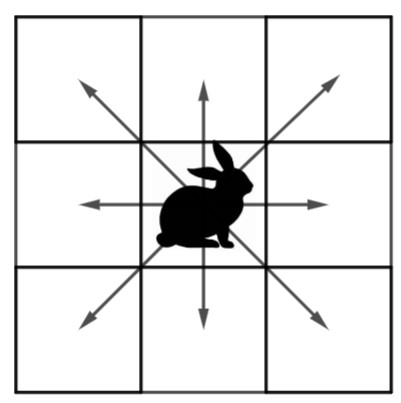
\includegraphics[max width=0.36\textwidth, alt={Осемте възможни хода на Зайо Байо към квадратчета с общ връх}, center]{assets/5-4-rabbit-moves.jpg}

а) Кумчо Вълчо при всеки свой ход се мести \textbf{два пъти последователно} от едно квадратче в съседно на него по страна. (На чертежа са показани три възможни хода на Кумчо Вълчо.)

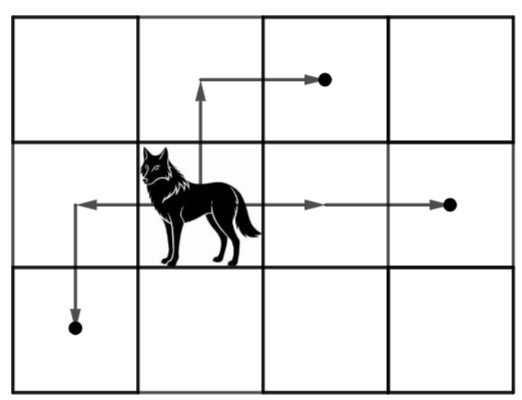
\includegraphics[max width=0.48\textwidth, alt={Три възможни хода на Кумчо Вълчо с две последователни премествания}, center]{assets/5-4-wolf-two-steps.jpg}

Докажете, че както и да застанат в началото върху дъска $2024\times2024$, Зайо Байо винаги може да избяга от Кумчо Вълчо, без да напусне дъската.

б) При всеки свой ход Кумчо Вълчо се мести \textbf{един или два пъти} от едно квадратче в съседно на него по страна. (На чертежа са показани четири възможни хода на Кумчо Вълчо.)

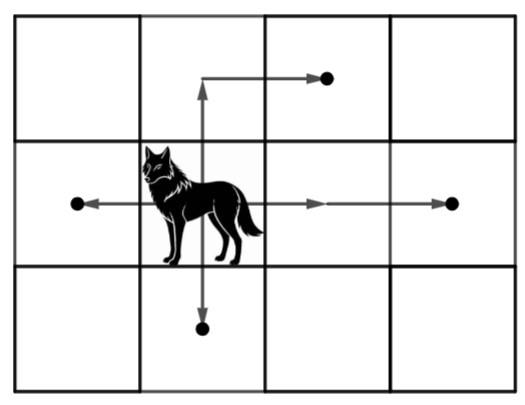
\includegraphics[max width=0.48\textwidth, alt={Четири възможни хода на Кумчо Вълчо с едно или две премествания}, center]{assets/5-4-wolf-one-or-two-steps.jpg}

Докажете, че ако дъската е безкрайна, Зайо Байо винаги може да избяга от Кумчо Вълчо.

Решение. а) Да оцветим дъската шахматно. Можем да забележим, че при всеки свой ход, състоящ се от две премествания в съседно по страна квадратче, Кумчо Вълчо отива в квадратче с един и същ цвят.

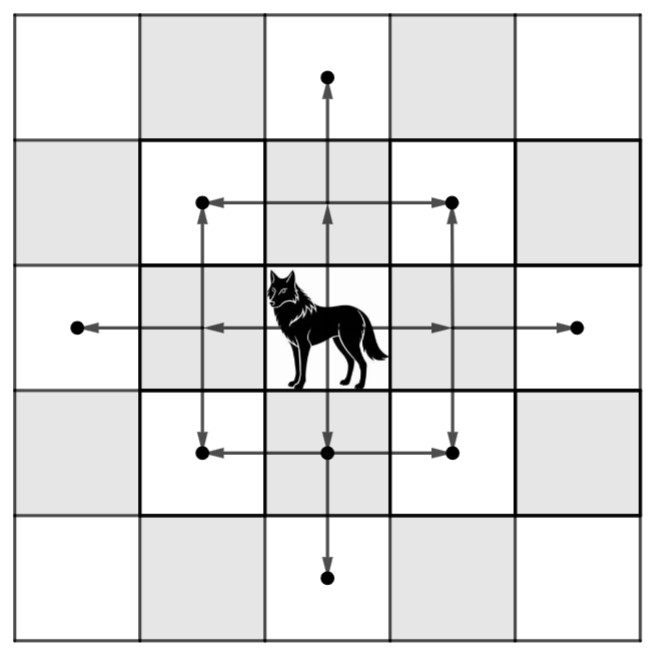
\includegraphics[max width=0.62\textwidth, alt={Шахматно оцветяване и възможните крайни квадратчета след хода на Кумчо Вълчо}, center]{assets/5-4-checkerboard-strategy.jpg}

Зайо Байо обаче може да смени цвета на квадратчето, в което е (с преместване нагоре, надолу, наляво или надясно) или да не го променя (с преместване по диагонал). Зайо постъпва по следния начин:

• ако в началото цветът на квадратчето му е като този на Кумчо Вълчо, той сменя цвета при първия си ход и след това да се движи само по диагонал;

• ако в началото цветът на квадратчето му е различен от този на Кумчо Вълчо, се движи само по диагонал.

Така и в двата случая след всеки ход Зайо Байо и Кумчо Вълчо ще са в квадратчета с различен цвят, следователно Зайо никога няма да бъде хванат.

б) Ще наричаме \emph{опасна територия} ромба, състоящ се от квадратчетата, в които Кумчо Вълчо може да попадне при следващия си ход. На чертежа опасната териотория е оцветена в сиво.

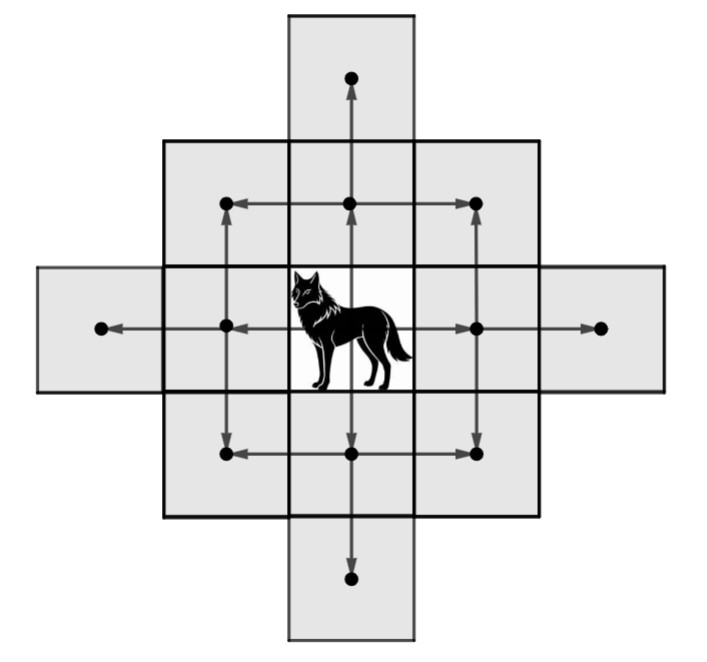
\includegraphics[max width=0.62\textwidth, alt={Опасната територия около Кумчо Вълчо, оцветена в сиво}, center]{assets/5-4-danger-zone.jpg}

Ако заекът се намира в опасната територия, с един ход по диагонал той може да излезе от нея. Тогава вълкът на следващия си ход не може да го хване.

Ако заекът се намира извън опасната територия, винаги може да направи такъв ход, че да не влезе в нея (дъската е безкрайна). Така вълкът на следващия си ход не може да го хване и заекът може да бяга безкрайно.

Ето една примерна стратегия на заека:

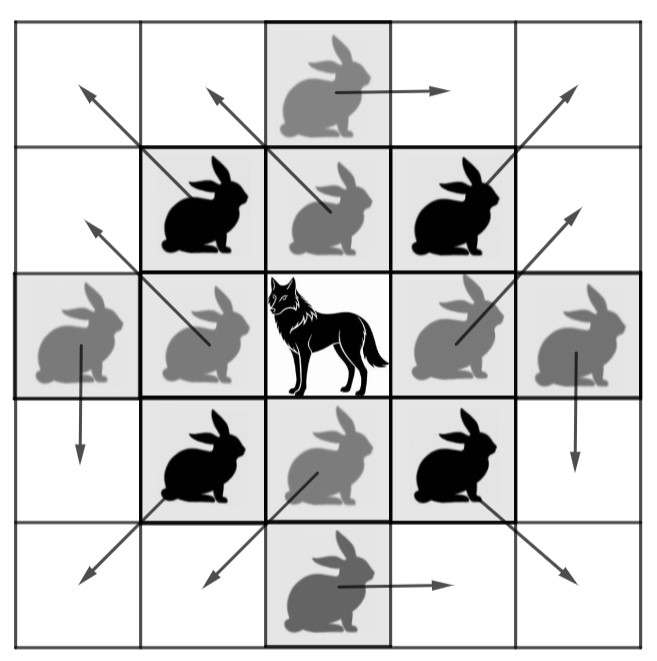
\includegraphics[max width=0.62\textwidth, alt={Примерна стратегия на заека спрямо променящата се опасна територия}, center]{assets/5-4-example-strategy.jpg}

След всеки ход на вълка опасната територия се променя и заекът трябва да действа според горепосочената стратегия.

Оценяване. а) Пълно решение: 4 точки.

За шахматно оцветяване – 1 точка.

За стратегия, ако Вълчо и Зайо са на едноцветни полета – 1 точка.

За стратегия, ако Вълчо и Зайо са на едноцветни полета – 1 точка.

За коментар защо Зайо винаги може да реагира – 1 точка.

За конкретна стратегия без доказателство: в зависимост от обосновката, до 2 точки.

б) Пълно решение: 3 точки.

За определяне на опасната територия – 1 точка.

За довършване – 2 точки.
